%#!platex main.tex

\section{Fractal}

\emph{フラクタル}(fractal)は数学者ブノワ・マンデルブロ(Benoit
B. Mandelbrot)が提唱した幾何学の概念である.フラクタル図形と呼ばれる図形
は自己相似性を持ち, 図形のどこを拡大しても全体と同じ形を見ることができる.
図\ref{fig:gasket}は\emph{シェルピンスキーのギャスケット}と呼ばれるフラ
クタル図形である.三角形を一定の法則に基づいて分割していくことで,無限に
続いていく三角形が得られる.その形はどこを拡大しても同様の法則性を持った
図形が得られる.また,自然界の多くの場面でもフラクタル構造をみることがで
きる. 海岸線や, シダ植物などにもフラクタル構造をみることができる. フラク
タルを考えることは自然科学研究の新たなアプローチとしても発展した.

自己相似性を持つ図形はフラクタルという名がつけられる以前から研究されてい
たが, 名が付けられることで, 研究が進むことになった. しかし, こうした図形
達に名が付けられたことに加え, コンピュータの普及により様々なフラクタル図
形を計算, 描画することができるようになり,アートとしても大きく発展した.

フラクタルの特異な形状は多くの人々の興味を引き, アートとしても大きく発展
した. これにはコンピュータの普及も大きく関連しており, コンピュータ文化と
の関連は切り離せない. フラクタルに関するコミュニティとして最大ともいえる
ウェブサイトに, Fractal Forum\footnote{Fractal Forum:
\url{http://www.fractalforums.com/}}がある. この章でこのコミュニティから
生れたフラクタル図形や描画手法は多く, この章で紹介するフラクタルも
Fractal Forumから生れた. これらのフラクタルは数学的な研究対象にならない
ものが多いものの, アートとしては非常に興味を引く形状を持つ.

また,\emph{デモシーン}({\it Demoscene})という文化もフラクタルレンダリン
グと関連が深い.
デモシーンは\emph{デモ}({\it Demo})と呼ばれるリアルタイ
ムにCGグラフィクスや音楽を生成するプログラムを見せ合うコンピューターサブ
カルチャーの一つである.美しいコンピュータグラフィクスを効率よく,さらに
小さなサイズのプログラムで描画することを追求しており, 数式で複雑な形状を
描画できるフラクタルと相性が良い.
また, デモからは様々な最適化手法をみることができる.
 デモシーンに関しては,Demoscene - The
 Art of the Algorithm\footnote{Demoscene - The Art of the Algorithms:
 \url{https://www.youtube.com/watch?v=iRkZcTg1JWU}}というドキュメンタリー
 が詳しい.
著名なデモシーナーのInigo Quilez(iq)は自身のウェブページ\footnote{Inigo
Quilez's webpage: \url{http://iquilezles.org/index.html}}にコンピュータグラフィ
 クスに関する様々な記事をまとめている.
 ここで紹介する手法もまとめられているので, 合せて参考にされたい.

 この章では, 後のクライン群の可視化に関わりのあるフラクタルとその描画手
 法についてまとめる.
 ここで述べたもの以外にも様々なフラクタル図形が存在している.
 それらについてはマンデルブロ自身の著作である\cite{fractal}に網羅的にま
 とめられている.

\begin{figure}[htbp]
 \center
 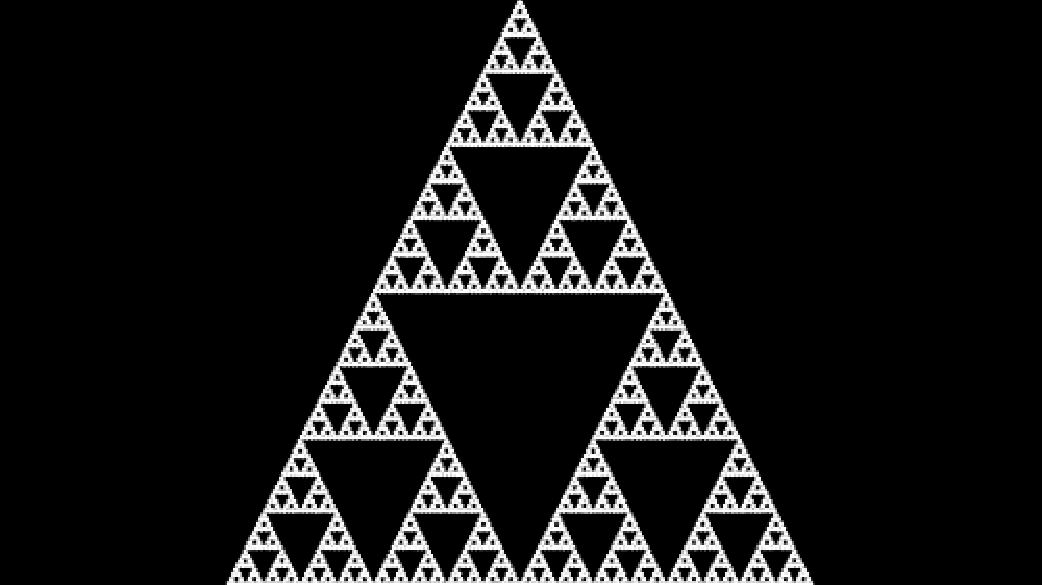
\includegraphics[width=3in, height=3in, keepaspectratio]{../img/fractal/gasket.pdf}
 \caption{Sierpinski gasket}
 \label{fig:gasket}
\end{figure}

\subsection{Shader Based Rendering}

この節では,近年よく使われるシェーダを用いたレンダリング手法について触れる.
最近のデモ作品でよく用いられる作品制作手法の1つに\textit{OpenGL Shading
Language(GLSL)}や\textit{High Level Shading Language(HLSL)}の\emph{フラ
グメントシェーダ}(Fragment Shader)を用いるものがある.
フラグメントシェーダは本来,ポリゴンに陰影をつけるために使用され, その処
理はGPUで行なわれる.
GPUは浮動小数演算性能に優れていることに加え,各ピクセルの演算は並列に行
われるため高速である.

この手法では, スクリーンスペースに矩形のポリゴンをレンダリングすることで
\emph{プロシージャル}(\textit{Procedural})に図を描画する.
プロシージャルとは, 数式やアルゴリズムを用いて形状を生成すること等を
指す.
複雑な形状をポリゴンで表現するよりもプログラムの実行サイズを下
げたり, 計算速度を向上させたりすることができるため, デモの, 小さなプログ
ラムサイズでリアルタイムにレンダリングするという目的に適している.
フラクタルはしばしば簡潔なアルゴリズムで複雑な形状を生成するので, デモに
おいてもよく使われる.

アルゴリズム\ref{shaderSample}に擬似コードと図\ref{fig:simpleShader}にレ
ンダリング結果を示した.
このように, ピクセルごとに座標が与えられるので, これを用いてピクセルの色
を決定する.

\begin{algorithm}
 \begin{algorithmic}
  \begin{minipage}{0.5\hsize}
   \caption{Sample Shader}
   \label{shaderSample}
   \REQUIRE COORDINATES, resolution
   \STATE uv = COORDINATES / resolution
   \STATE COLOR = Vector3(uv.x uv.y, 1.)
  \end{minipage}
 \end{algorithmic}
\end{algorithm}

幾何図形を描く際には多くの場合, 距離関数を用いる.
距離関数は, 図形からの最短距離を返す関数である.
原点中心,半径$r$の円の距離関数は以下のようになる.
\begin{align*}
 f(z) =  length(z) - r
\end{align*}
この関数は円周からの距離を返す.
座標が, 負の距離をもつときに色をつけるような処理を書く
と円を描くことができる.
アルゴリズム\ref{renderCircle}に疑似コードと図\ref{fig:circleShader}にレ
ンダリング結果を示した.
複数の図形を描きたい時は,複数の距離関数を評価し,最も小さな距離を求めれ
ばよい.

\begin{algorithm}
 \begin{algorithmic}
  \caption{Render circle}
  \label{renderCircle}
  \REQUIRE COORDINATES, resolution
  \STATE p = COORDINATES - (resolution / 2.)
  \STATE distance = length(p) - radius
  \IF{distance $\leq$ 0}
  \STATE COLOR = Vector3(1, 1, 1)
  \ELSE
  \STATE COLOR = Vector3(0, 0, 0)
  \ENDIF
 \end{algorithmic}
\end{algorithm}

 \begin{figure}[htbp]
  \begin{minipage}{0.5\hsize}
   \center
   
\includegraphics[ height=1.5in, keepaspectratio]{../img/fractal/uv.pdf}
   \caption{Simple shader}
   \label{fig:simpleShader}
  \end{minipage}
  \begin{minipage}{0.5\hsize}
   \center
   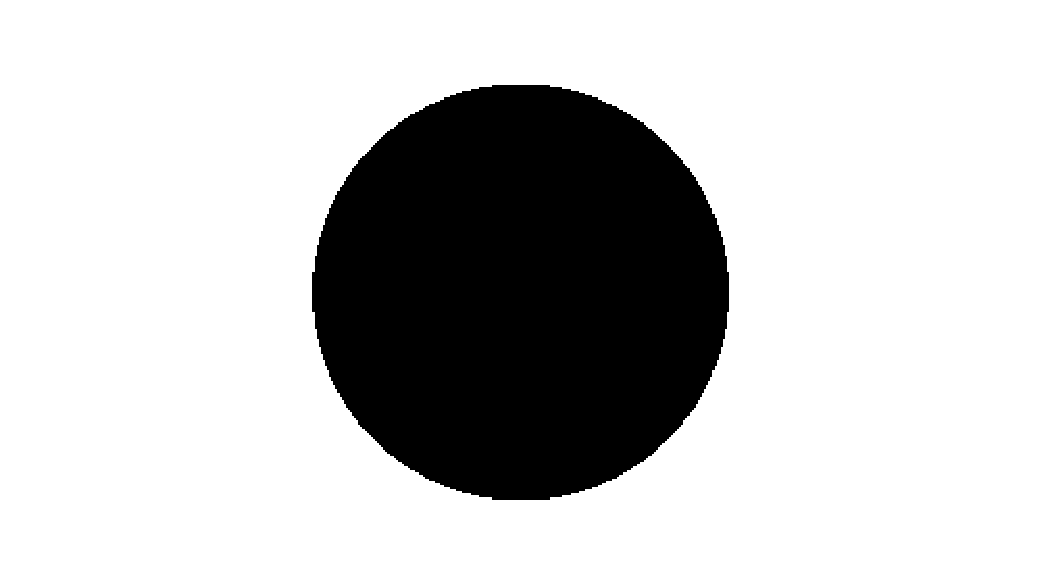
\includegraphics[ height=1.5in, keepaspectratio]{../img/fractal/circle.pdf}
   \caption{Circle}
   \label{fig:circleShader}
  \end{minipage}
 \end{figure}

シェーダを用いたレンダリングはglslsandbox\footnote{glslsandbox:
\url{http://glslsandbox.com/}}やShadertoy\footnote{Shadertoy:
\url{https://www.shadertoy.com/}}といったウェブサービスで手軽に試すこと
ができる.
doxasによるwgld\footnote{wgld: \url{https://wgld.org/d/glsl/}}には,シェー
ダによるレンダリングの入門事項がよくまとまっている.

また,GPUの計算性能をより汎用的な計算に用いるためのプラットフォームとしてCUDA
やOpenCLが登場している.
これらのプラットフォームを用いることでシェーダではできない複雑な処理を
GPUで行うことができるようになり,GPUによる並列演算は機械学習などの分野に
も活躍の場を広げた.
このようにGPUによる演算を画像処理以外の汎用的な用途に用いる技術は
\textit{GPGPU(General-purpose computing on graphics processing units)}
と呼ばれている.

\subsubsection{Distance Estimation}

また,距離関数は陰関数から近似的に導出することができる.
この手法を\textit{Distance Estimation}とよぶ.
iqによる式\footnote{distance estimation:
\url{http://iquilezles.org/www/articles/distance/distance.htm}}
のひとつを紹介する.

平面上のある点を$x$, $e$を$x$から最も近い零点集合へ向うベクトルとすると,
零点集合上の点は$x + e$と表せる.
求めたい距離は$|e|$となる.
$f(x + e) = 0$から導出してみよう.
これをテイラー展開すると
$f(x + e) = f(x) + f'(x) \cdot e  + \frac{1}{2}f''(x) \cdot e^2 ...$とな
る. ここで$e$が十分に小さいと仮定し, 2次以上の項を無視する線型近似を行うと
$0=|f(x + e)| \approx |f(x) + f'(x) \cdot e|$
となる. ここで, $x, e$はベクトルであり, $\cdot$は内積を表すことに注意す
る.
三角不等式によって, $| f(x) + f'(x) | \geq |f(x)| - |f'(x)|$であるから,
$0 \geq |f(x)| - |f'(x) \cdot e|$.
また, コーシーシュワルツの不等式より,
$|f'(x)| \cdot |e| \geq | f'(x)\cdot e|$
であるから,
$0 \geq |f(x)| - |f'(x) \cdot e| \geq |f(x)| - |f'(x)| \cdot |e|$
となる.
最後に$0 \geq |f(x)| - |f'(x)| \cdot |e|$を変形すると
$|e| \geq \frac{|f(x)|}{|f'(x)|}$が得られる.
このことから, ある点$x$に対して, 陰関数$f(x)$が表す零点集合への最短距離を返す近
似関数は以下のように表すことができる.
\begin{align*}
 DistanceFunction(x) \approx \frac{|f(x)|}{|\bigtriangledown f(x)|}
\end{align*}
ただし, $e$が十分小さいことを仮定しているため, 零点集合から遠い点につい
ては誤差が大きくなってしまうことに注意する.
導関数から得られた微分値の代わりにヤコビアンが用いられたり, 中心差分法等
で導出された微分の近似値が用いられることもある.

\subsubsection{Ray tracing}

シェーダのみで三次元形状を描画する際には\emph{レイトレーシング}({\it Ray
tracing})が用いられる.
レイトレーシングはあらかじめ設定された視点(カメラ)から
\emph{レイ}({\it Ray}, 光線)を飛ばし,
その挙動を計算することで物体を描画する手法である.
図\ref{fig:raytrace}にレイトレーシングの模式図を示した.
レイと物体の交差点はレイの原点と方向から代数的に計算することができる.

また,\emph{レイマーチング}({\it Ray marching, Sphere tracing}とも呼ばれ
る)\cite{sphereTracing}という手法で,物体の距離関数からレイとの交差点を
近似的に求めることができる.
図\ref{fig:raymarch}にレイマーチングの模式図を示した.
視点$P_0$に最も近い物体との距離を求め, その距離分だけレイを進め, その位
置を$P_1$とする.
この作業を繰り返し, 得られた点列の極限点が交差点となる.

また, レイマーチングでは, 距離関数をうまく組み合わせることで, 三次元形状
の和, 差, 積をとるような演算も高速に行なえる.
この手法はメッシュによらないプロシージャルな形状表現に適しており, デモシー
ンでも広く使われている.

交差点を代数的に計算することが難しいフラクタル形状をレンダリングする際に
は, Distance Estimationによって形状との距離を求めてレイマーチングを行な
うのが一般的である.

 \begin{figure}[htbp]
  \begin{minipage}{0.5\hsize}
   \center
   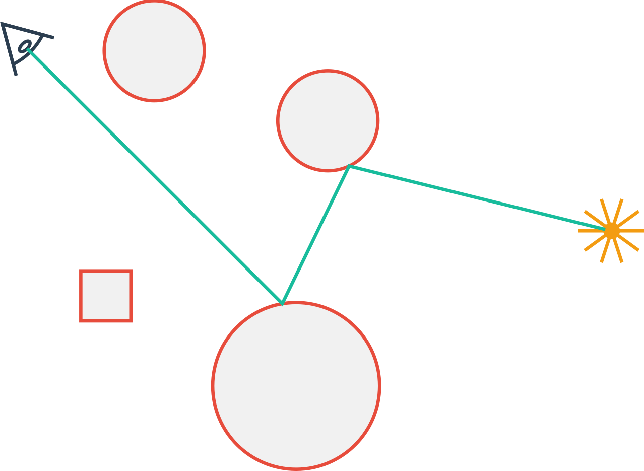
\includegraphics[width=3in, keepaspectratio]{../img/fractal/raytrace.pdf}
   \caption{Ray tracing}
   \label{fig:raytrace}
  \end{minipage}
  \begin{minipage}{0.5\hsize}
   \center
   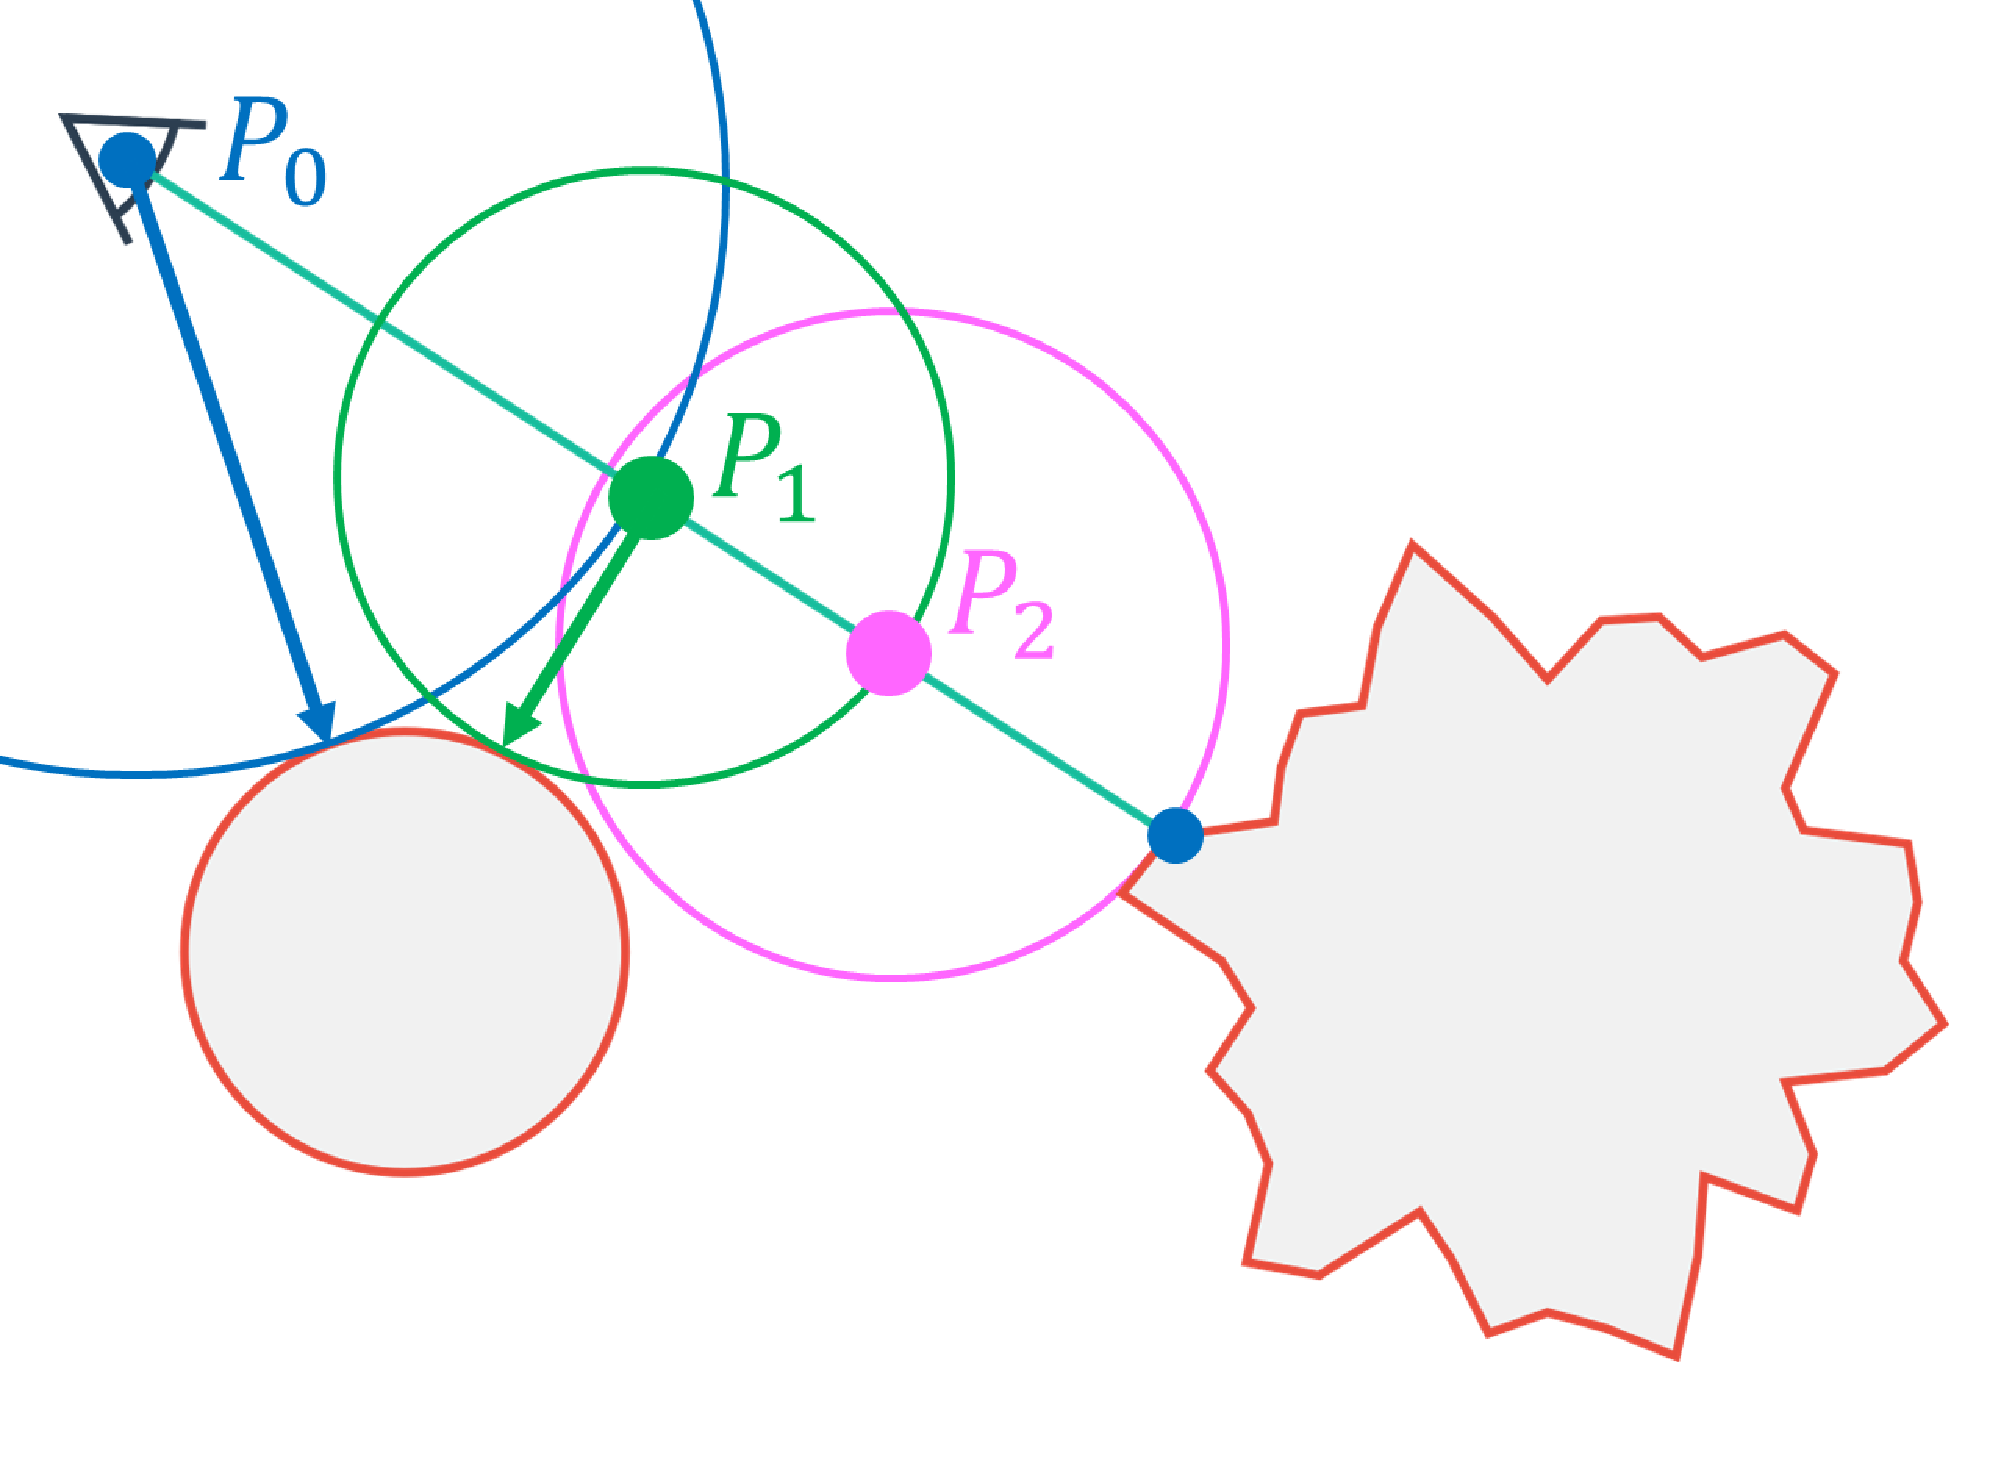
\includegraphics[width=3in, keepaspectratio]{../img/fractal/raymarching.pdf}
   \caption{Ray marching}
   \label{fig:raymarch}
  \end{minipage}
 \end{figure}

\subsection{Escape-time Fractals}

{\it Escape-time Fractals}は複素平面上の点に対して,特定の漸化式を計算し,
その点の軌道の収束,発散を見ることで描画されるフラクタルである.
Escape-time Fractalsで代表的なものが\emph{マンデルブロ集合}({\it
Mandelbrot set})である.
マンデルブロ集合の漸化式は以下のようになる.
\begin{eqnarray*}
 z, c \in \mathbb{C} \quad
 \begin{cases}
  z_{n+1} = z^2_{n} + c \\ z_0 = 0
 \end{cases}
\end{eqnarray*}
複素平面上の点$c$に対して, $\displaystyle \lim_{n \to \infty} z_n$が無
限大に発散しないものをマンデルブロ集合と呼ぶ.
図\ref{fig:mandelbrot}における黒い部分がマンデルブロ集合である.
その他の部分については, 発散と判定されるまでの計算の回数によって色をつけ
た.
マンデルブロ集合はその単純な式から驚くほど豊富なバリエーションの図を見る
ことができる.
その他のEscape-time fractalには,\emph{ジュリア集合}({\it Julia set})(図
\ref{fig:julia})や\emph{ファトゥー集合}({\it Fatou set})等がある.

各点における漸化式の計算はお互いに干渉しないので,そのままシェーダでの実
装が可能であるが,先に述べたDistance Estimationを用いることで,エイリア
シングノイズ等を避けてより精細に描画することができる.
これには{\it Green Function}と呼ばれる陰関数を用いる.
導出はiqによる記事\footnote{distance rendering for fractals:
\url{http://iquilezles.org/www/articles/distancefractals/distancefractals.htm}}
が詳しい.
Green Functionに関しては,マンデルブロ集合に関する詳細な議論となってしま
うので,\cite{mandelbrot}を参考にされたい.

\begin{figure}[htbp]
 \begin{minipage}{0.49\hsize}
  \begin{center}
   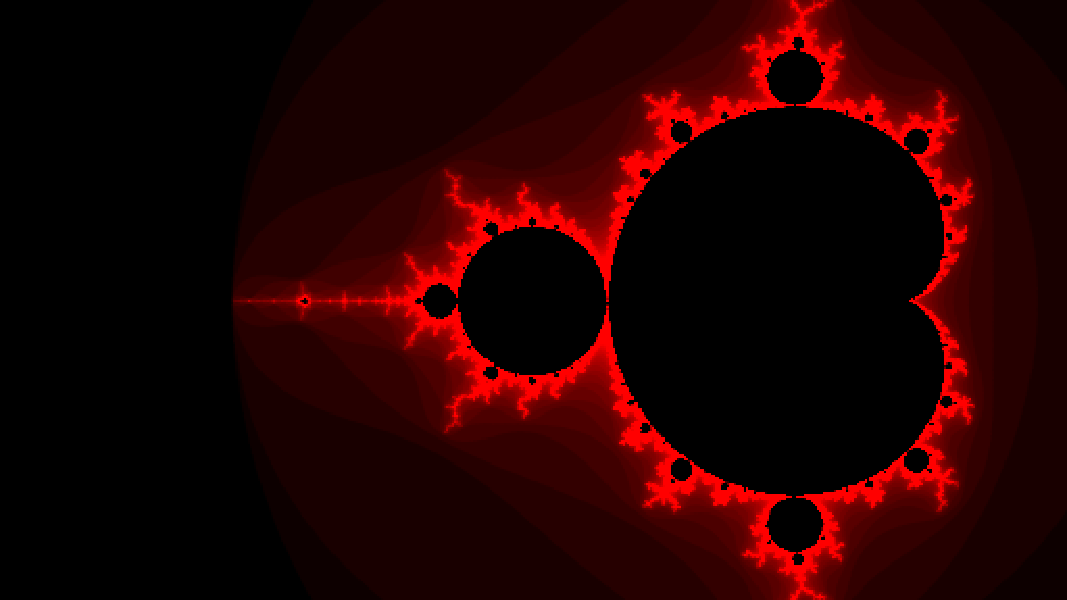
\includegraphics[width=3in, height=3in, keepaspectratio]{../img/fractal/mandelbrot.pdf}
   \caption{Mandelbrot set}
   \label{fig:mandelbrot}
  \end{center}
 \end{minipage}
 \begin{minipage}{0.49\hsize}
     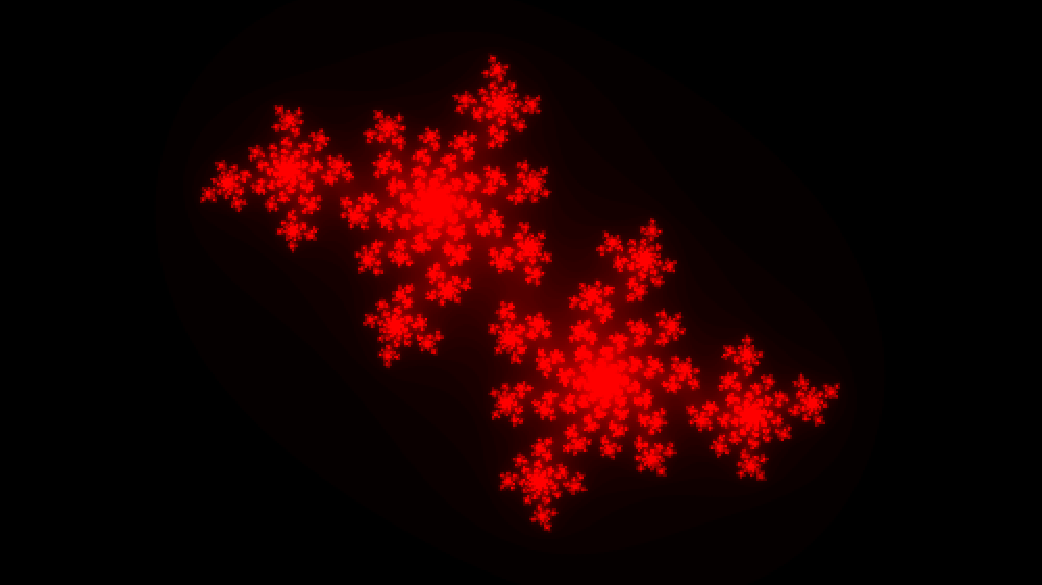
\includegraphics[width=3in, height=3in, keepaspectratio]{../img/fractal/julia.pdf}
   \caption{Julia set}
   \label{fig:julia}
 \end{minipage}
\end{figure}

\subsection{Distance Estimated 3D Fractals}

マンデルブロ集合は数あるフラクタルの中でも特に複雑な形状を見せるものであった
ので, その三次元への拡張も古くから興味が持たれてきた.

例えば,ジュリア集合を四元数を用いて計算した
Quaternion Julia 3D fractal\cite{4djulia}が1989年に発表されている.
しかし, この形状は四元数による回転対称性をもつため, 形状が単純でフラクタ
ルコミュニティの満足のいくものではなかった.

そのような中で, 2003年に発表された阿原・荒木による4
次元クライン群の一種である{\it Quasi Fuchsian 3D
Fractals}\cite{sphairahedra}はある程度の複雑性を持った3次元フラクタルで
あったため,コミュニティに大きな影響を与えたと言われている.
このフラクタルに関しては後の章で触れる.

この時期から, コンピュータのグラフィクス性能が向上し, 三次元のフラクタ
ル図形をリアルタイムに描画することができるようになった.
例えば, 2004年にKeenan CraneはQuaternion JuliaをGPUによってリアルタイムに
描画している. \footnote{Ray Tracing Quaternion Julia Sets on
the GPU:
\url{https://www.cs.cmu.edu/~kmcrane/Projects/QuaternionJulia/}}.
iqは2007年にQuaternion Juliaをテーマにした4k intro(実行ファイルのサイズ
を4kb以内に抑えたデモ作品),
\textit{kindernoiser}\footnote{http://www.pouet.net/prod.php?which=32549}
を発表している.

その後,2009年に遂にマンデルブロ集合をうまく三次元に拡張した{\it
Mandelbulb}が開発された.
これを皮切りに, 次々と複雑な三次元フラクタルの式が開発された.
それらの多くはEscape-time fractalの一種であり,
Distance Estimationとレイマーチングを用いることで効率よくレンダリングす
ることができる.
これらのフラクタルの歴史と実装についてはMikael Hvidtfeldt Christensen
による一連の記事\footnote{Syntopia, Distance Estimated 3D
Fractals:\\ \quad \quad
\url{http://blog.hvidtfeldts.net/index.php/2011/06/distance-estimated-3d-fractals-part-i/}}
によくまとめられている.

これらのフラクタルをレンダリングするためのソフトウェアは{\it Mandelbulb
3D}\footnote{Mandelbulb 3D:
\url{http://mandelbulb.com/2014/mandelbulb-3d-mb3d-fractal-rendering-software/}}
や{\it Mandelbulber}\footnote{Mandelbulber:
\url{http://www.mandelbulber.com/}}が有名である.
{\it Fragmentarium}\footnote{Fragmentarium:
\url{http://syntopia.github.io/Fragmentarium/}}はシェーダベースのグラフィ
クスを開発するための環境である.
フラクタルのサンプルコードも豊富で学習に役立つ.
{\it Fractal Lab}\footnote{Fractal Lab:
\url{http://hirnsohle.de/test/fractalLab/}}はブラウザ上でGLSLを用いてフ
ラクタルをレンダリングすることができるウェブアプリケーションである.
この章で使われている図のいくつかはFractal LabとFragmentariumを用いてレン
ダリングした.

\subsubsection{Mandelbulb}

三次元の拡張において問題になるのは, 三次元空間において用いる代数である.
マンデルブロ集合の漸化式は複素数の乗算と加算で構成されている.
$z^2$は点$z$に原点中心の回転と拡縮を作用させ, 加算$z + c$は平行移動を作用さ
せる. これによって点の軌道を考えることができる.
そのため, 三次元空間の点において, 軌道を考えることができるような$z^2$の
意味付けが必要であった.

そのためのアプローチのひとつが四元数を用いたQuaternion Juliaであるが,
生成される図は対称的であり, あまり興味を引くものではなかった.

最終的にDaniel White(twinbee)とPaul Nylander
が2009年に開発したMandelbulbが三次元に拡張されたマンデルブロ集合として広
く知られることとなった.

Whiteは球面座標上で漸化式を計算するアプローチを提案
\footnote{\url{http://www.fractalforums.com/3d-fractal-generation/true-3d-mandlebrot-type-fractal/}}
した.
図\ref{fig:mandelbulb2}は$z_{n+1} = z_n^2 + c$を用いてレンダリングした結
果であるが,あまり複雑な形状は現れなかった.
しかし,その後Nylanderが式を高次の積を扱えるように拡張した.
図\ref{fig:mandelbulb8}は$z_{n+1} = z_n^8 + c $という式でレンダリングさ
れた形状であり,これがMandelbulbとして知られている.Whiteのウェブページ
\footnote{Skytopia:
\url{http://www.skytopia.com/project/fractal/mandelbulb.html}}には開発の
詳しい経緯がまとめられている.

また, Mandelbulbも通常のマンデルブロ集合と同様にDistance Estimationによっ
て形状への最短距離を求めることができ, これによってレイマーチングで描画す
ることができる.

\begin{figure}[h!tbp]
 \begin{subfigure}{0.49\hsize}
   \begin{center}
    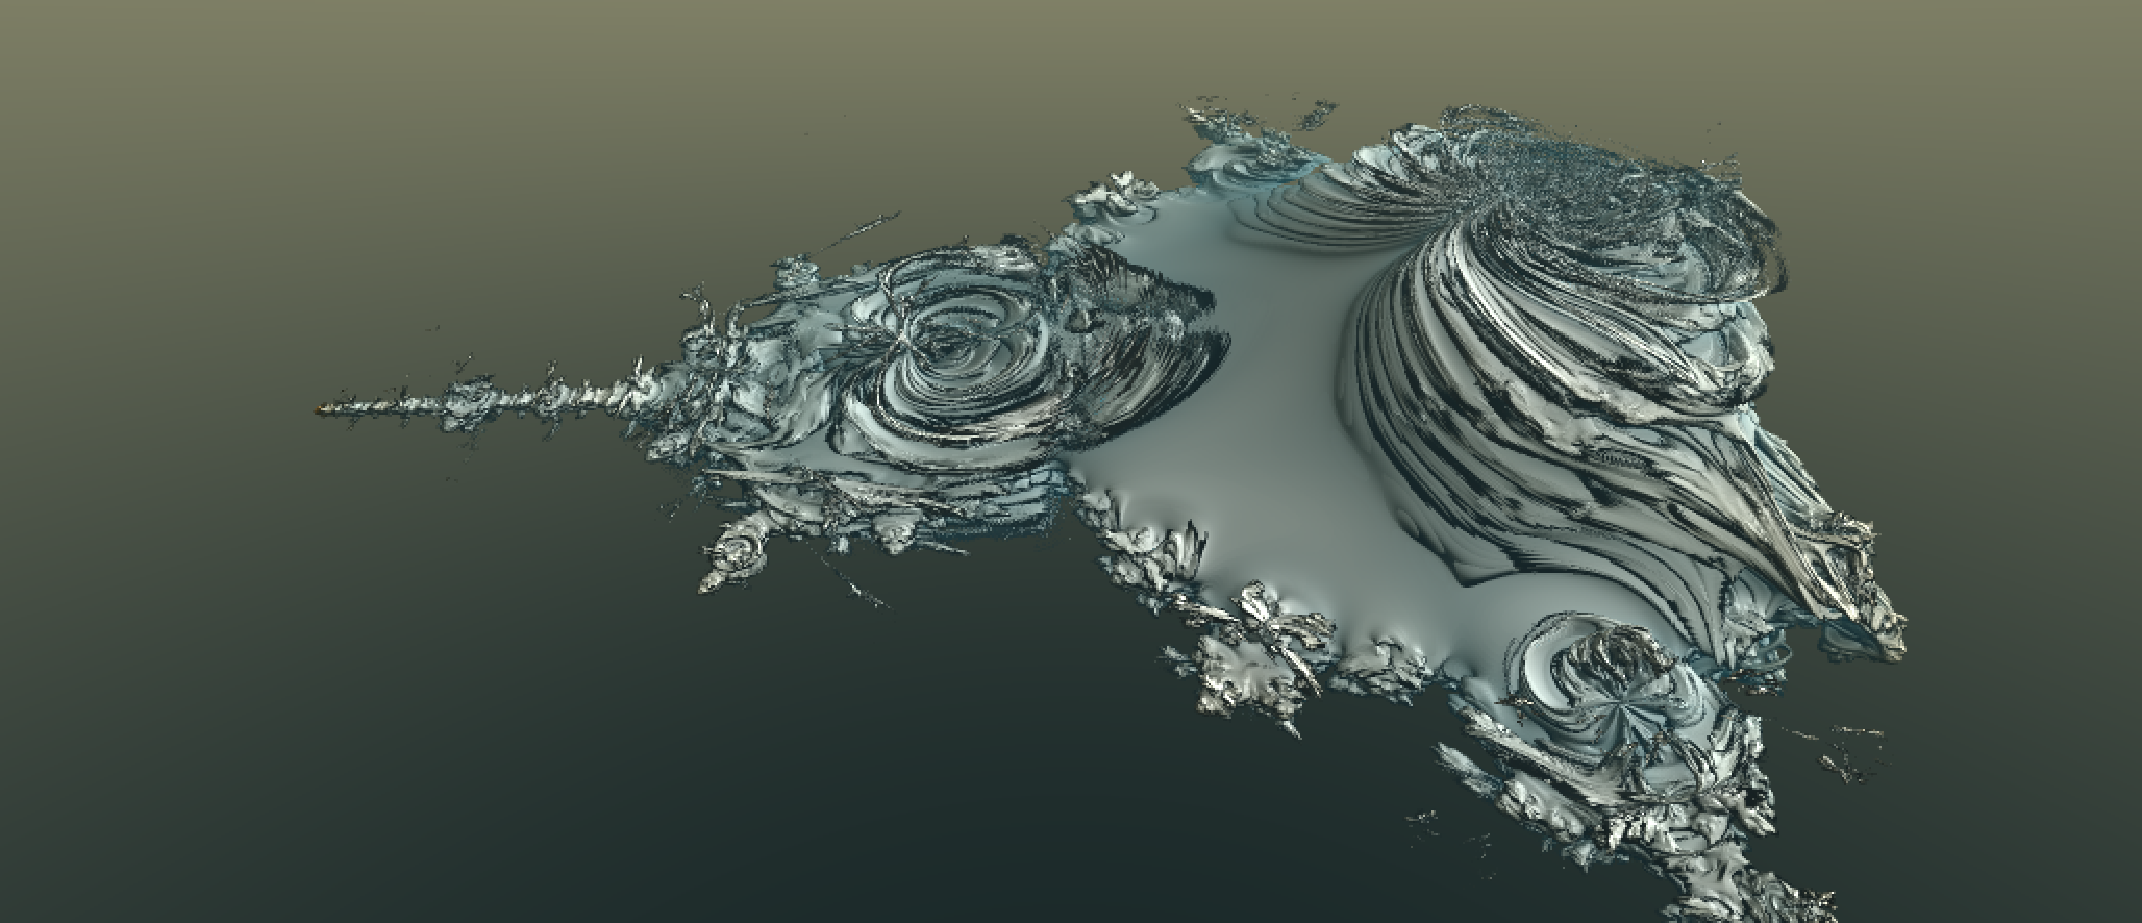
\includegraphics[width=3in, height=3in, keepaspectratio]{../img/fractal/mandelbulb2.pdf}
    \caption{$z_{n + 1} = z_n^2 + c$}
    \label{fig:mandelbulb2}
   \end{center}
 \end{subfigure}
 \hspace*{\fill}
 \begin{subfigure}{0.49\hsize}
   \begin{center}
    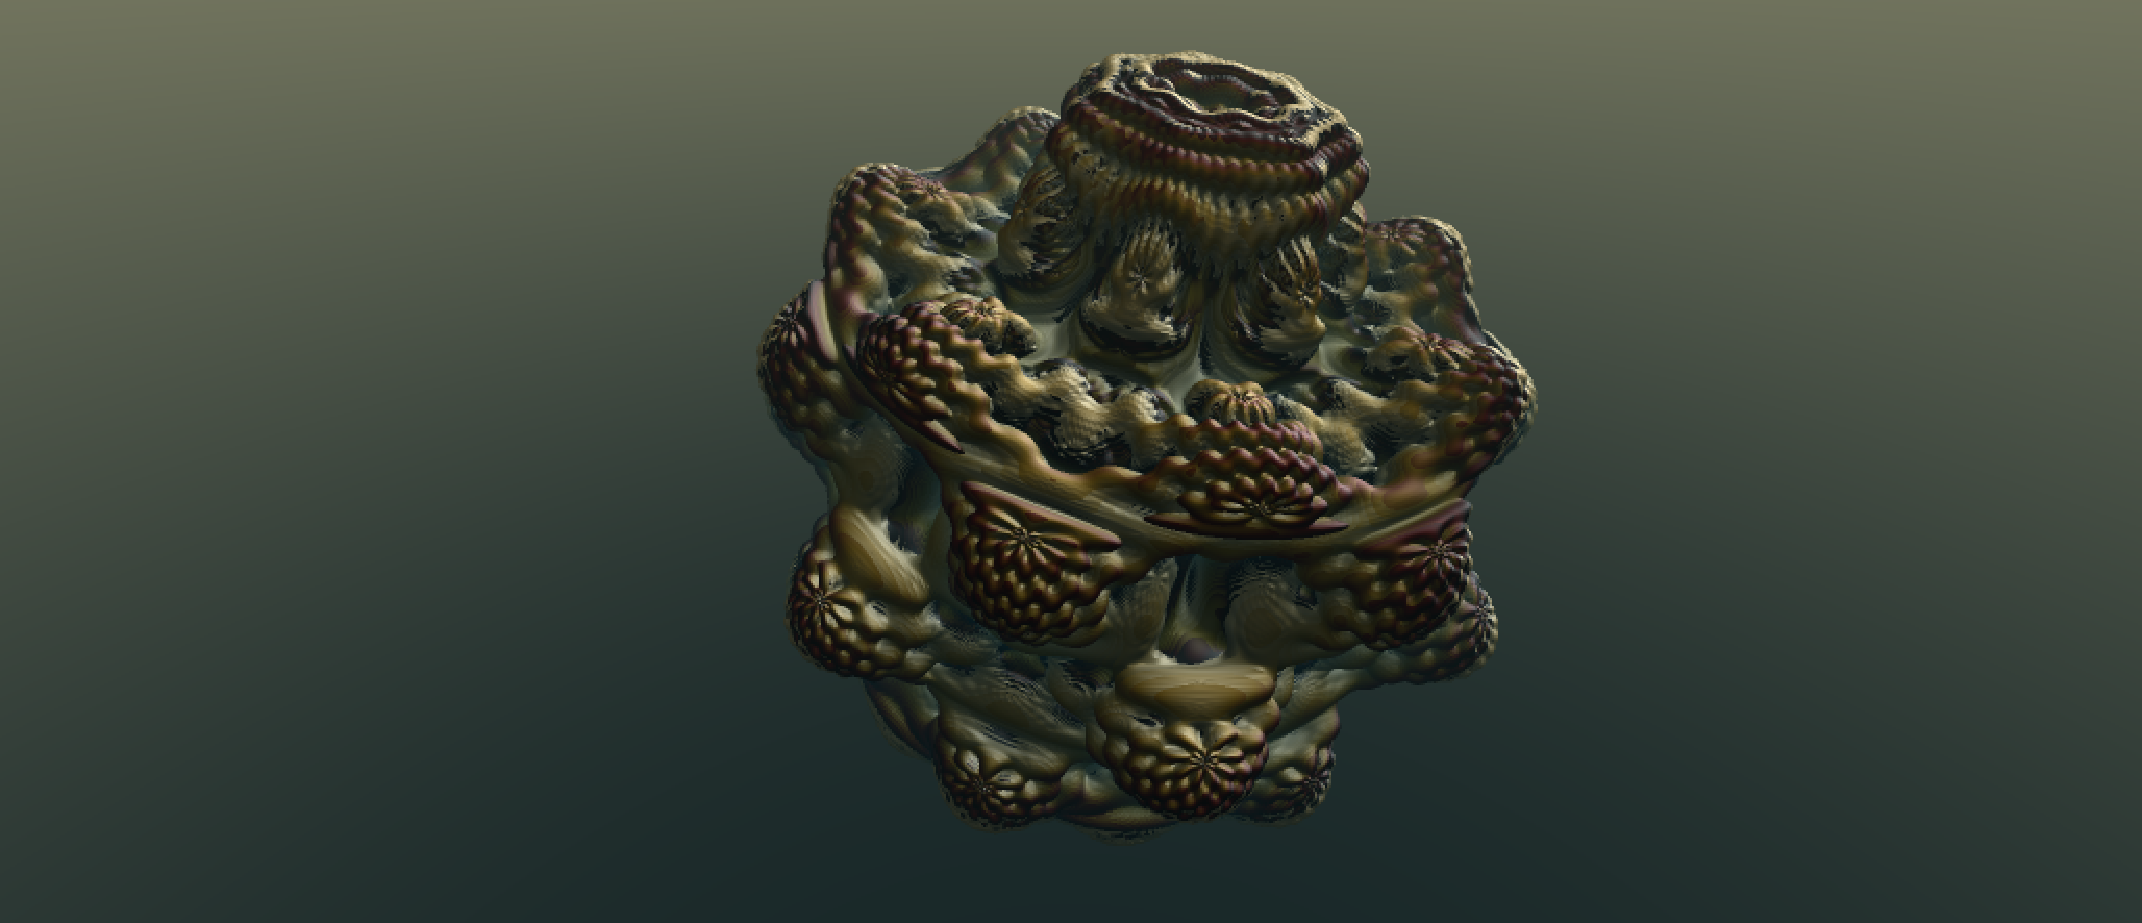
\includegraphics[width=3in, height=3in, keepaspectratio]{../img/fractal/mandelbulb8.pdf}
    \caption{$z_{n+1} = z_n^8 + c$}
    \label{fig:mandelbulb8}
   \end{center}
 \end{subfigure}
 \caption{Mandelbulb rendered by Fractal Lab}
\end{figure}

\subsubsection{Mandelbox}

その後,2010年にTom Loweによって{\it Mandelbox}\footnote{Mandelbox:
\url{https://sites.google.com/site/mandelbox/what-is-a-mandelbox}}が開発
された.
Mandelboxも三次元空間におけるEscape-time fractalである.
漸化式は$z_{n+1} = scale * spherefold(minR, boxfold(z_n)) + c$と表わせる.
ここで, {\it boxfold}は$x=\pm1, y=\pm1, z=\pm1$を頂点にもつ立方体の各面
に対して, 点が外側にある場合にその面に関する反転を行なう操作である.
また, {\it spherefold}は以下の式で定義される.
\begin{align*}
 spherefold(r, z) = \begin{cases}
                  \frac{z}{r^2} & 0 \le |z| < r \\
                  \frac{z}{|z|^2} & r \le |z|
                 \end{cases}
\end{align*}
基本は原点中心, 半径$r$の球に関する反転であるが値に制限を設けている.
球の反転は, 中心付近を無限遠点付近へと移してしまうため, 漸化式の計算途中
に中心付近を通る点が発散と判定されてしまう.
そこでspherefoldでは, 中心付近の点の反転をあらかじめ決めておいた最小の半
径における反転で置きかえることで軌道が発散しないようにしている.

MandelboxのDistance Estimationでは漸化式の微分としてヤコビアンの積を用いる.
式の各操作のたびに, ヤコビアンを累積していき,
最終的な点の原点からの距離をヤコビアンの積で割ることで距離を近似的に求
めることができる.

\begin{figure}[h!tbp]
 \begin{subfigure}{0.49\hsize}
   \begin{center}
    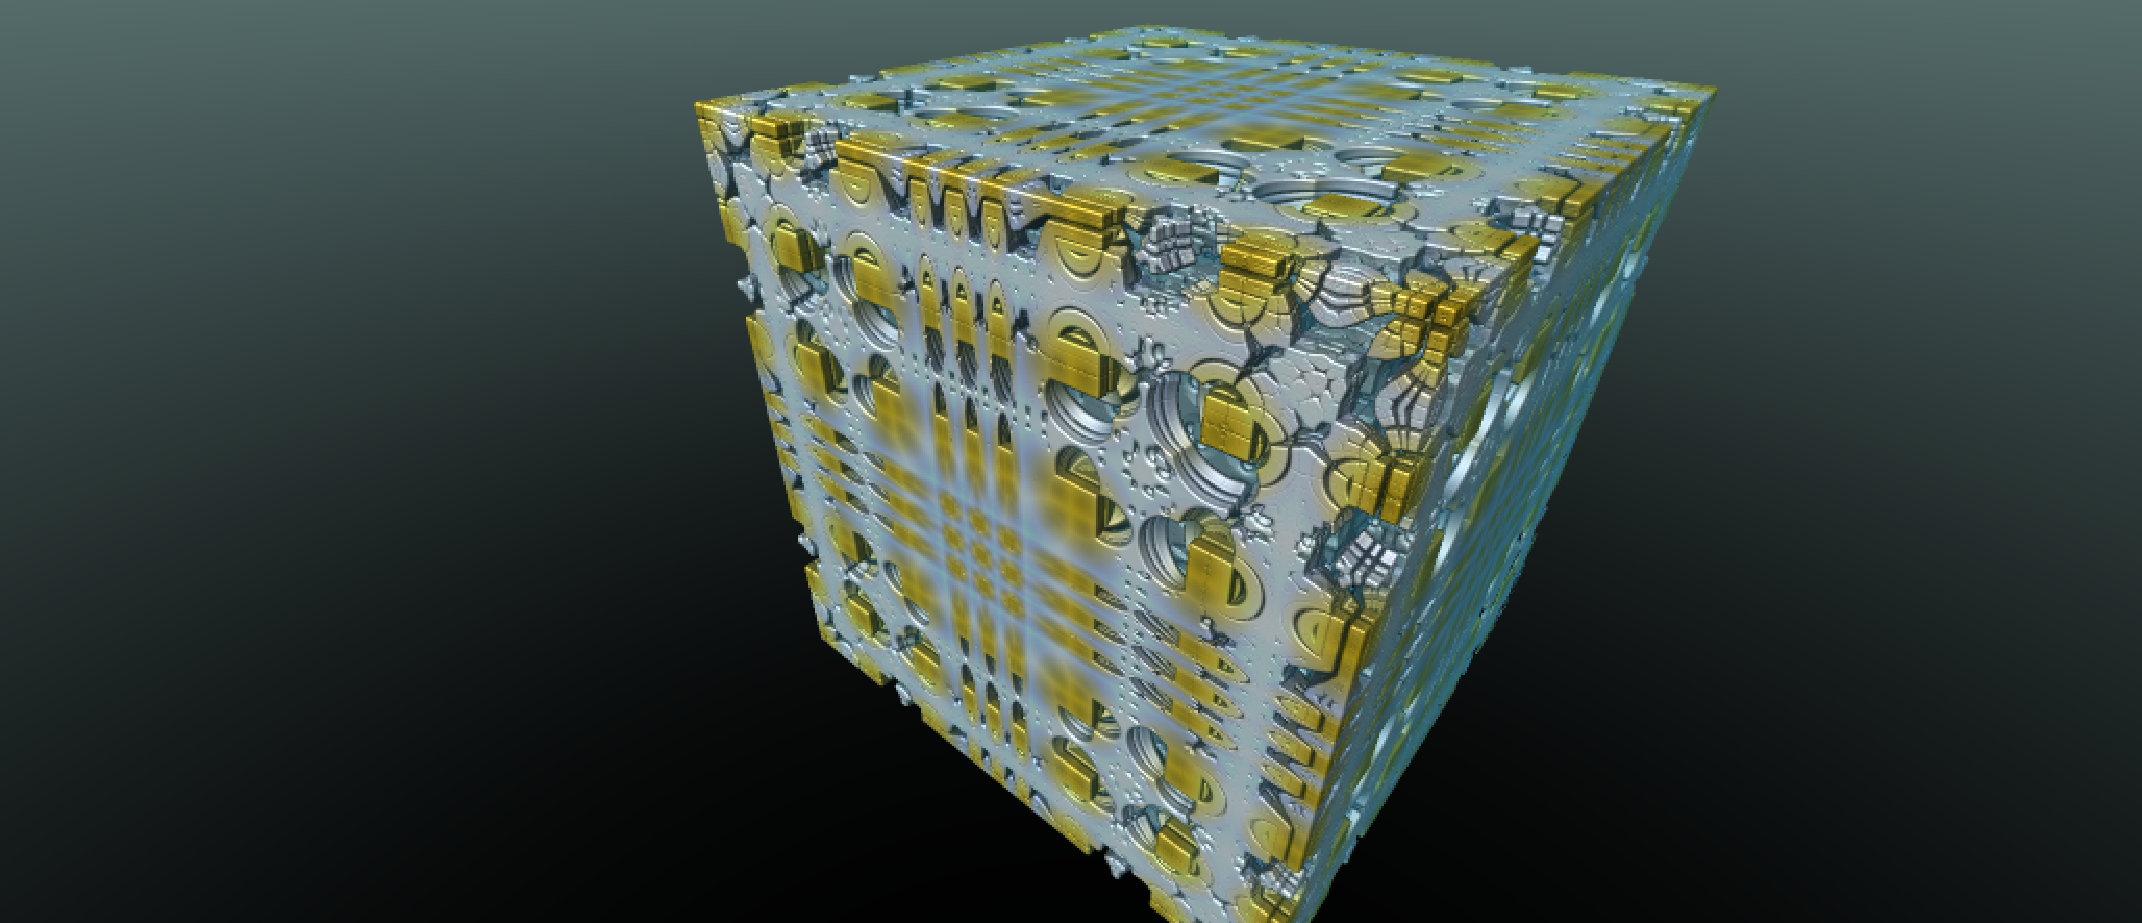
\includegraphics[width=3in, height=3in, keepaspectratio]{../img/fractal/mandelbox.pdf}
    \caption{}
    \label{fig:mandelbox1}
   \end{center}
 \end{subfigure}
 \hspace*{\fill}
 \begin{subfigure}{0.49\hsize}
   \begin{center}
    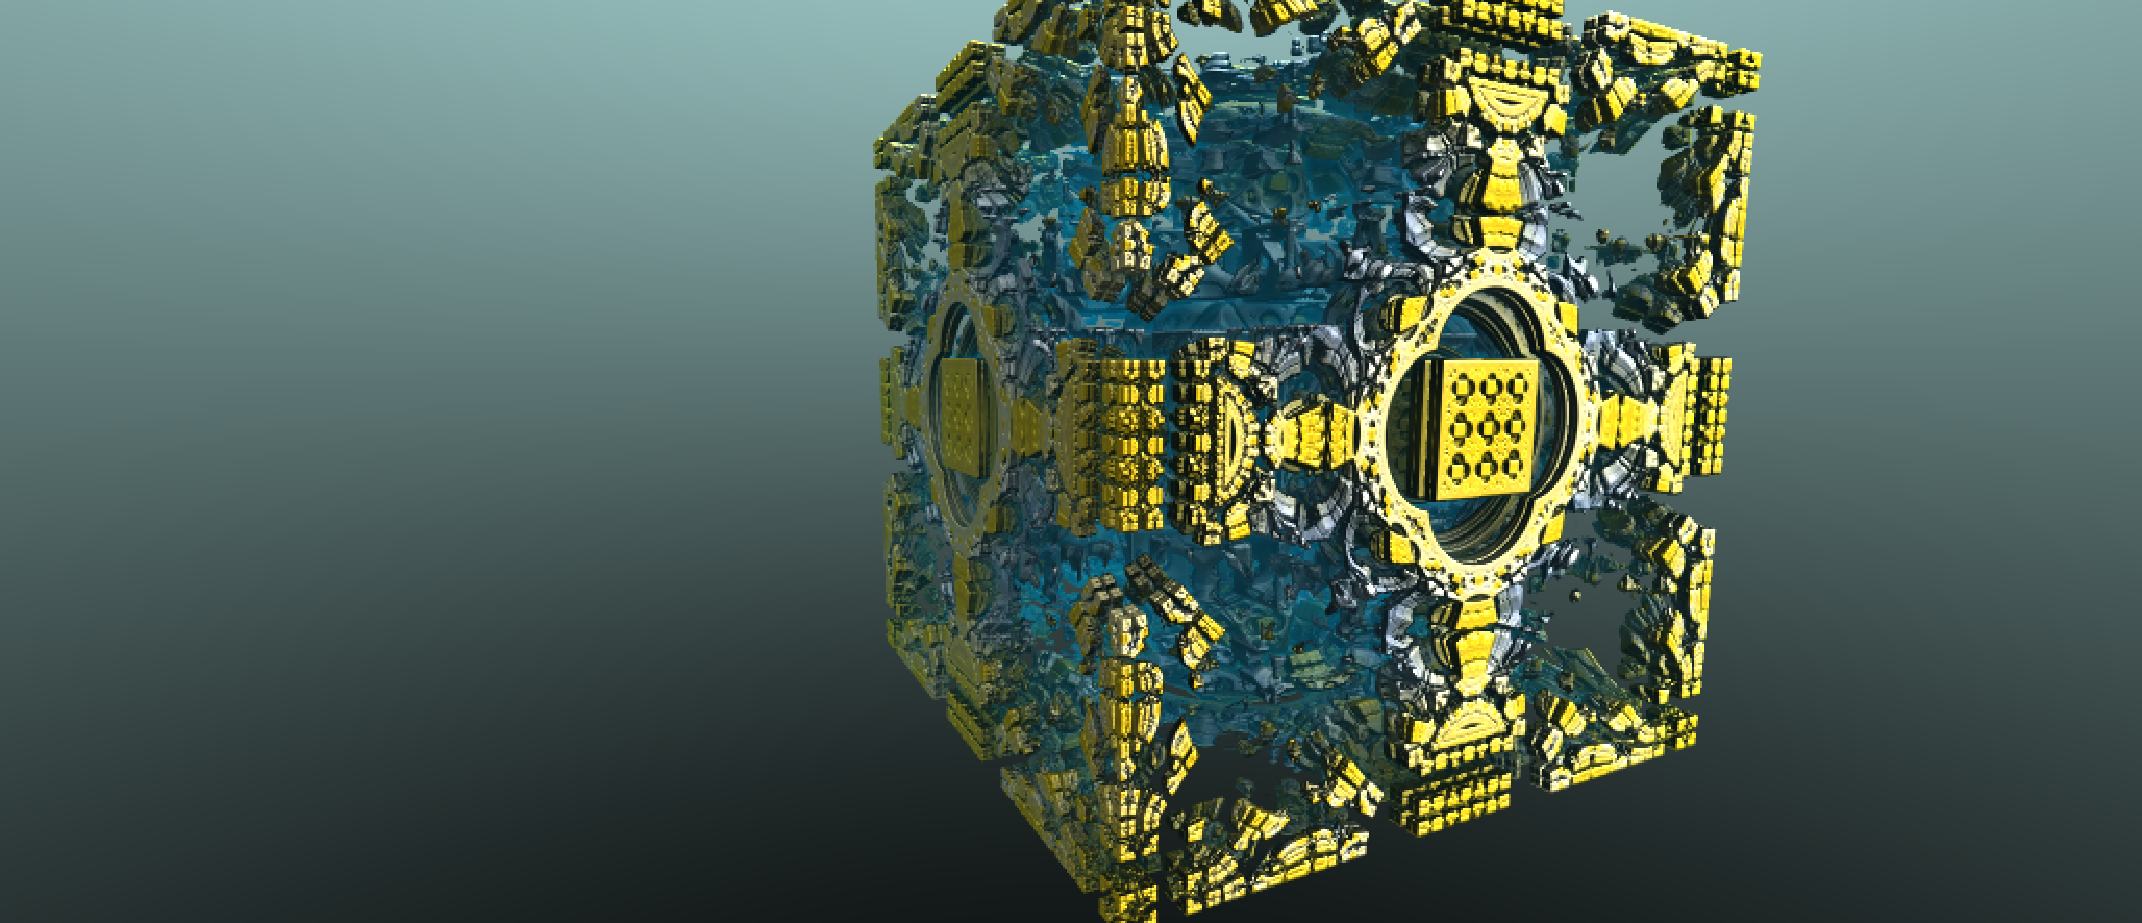
\includegraphics[width=3in, height=3in, keepaspectratio]{../img/fractal/mandelbox2.pdf}
    \caption{}
    \label{fig:mandelbox2}
   \end{center}
 \end{subfigure}
 \caption{Mandelbox rendered by Fractal Lab}
 \label{fig:mandelbox}
\end{figure}


\subsubsection{Pseudo-Kleinian}

Mandelboxの登場以降は漸化式にMandelbulbやMandelboxを含む複数の式を用いた
{\it Hybrid System}によって,様々なフラクタル作品が作られている.
興味深いHybrid Systemの1つに{\it pseudo-kleinian}がある.
これは球の反転に近い操作であるSpherefoldと平行移動と同じような働きをする
boxfoldの組み合わせによってクライン群のような形状が得られる式である.
図\ref{fig:pseudoKleinian}はFragmentariumのサンプルスクリプトを用いてレンダリングされた.

\begin{figure}[htbp]
  \begin{center}
   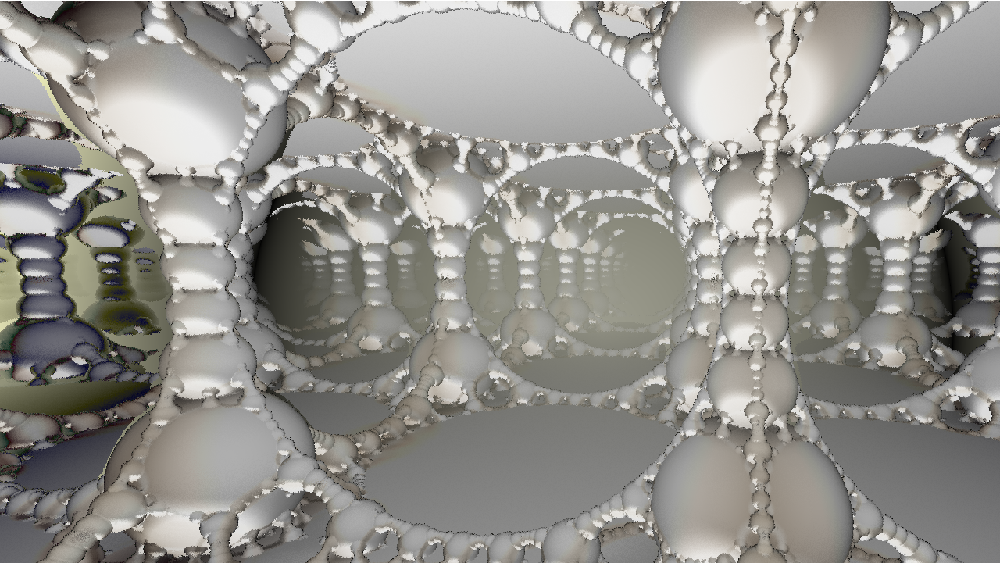
\includegraphics[width=3in, height=3in, keepaspectratio]{../img/fractal/pseudoKleinian.pdf}
   \caption{pseudo-kleinian}
   \label{fig:pseudoKleinian}
  \end{center}
\end{figure}


\subsection{Coloring by Orbit Trap}

フラクタルのレンダリングにおいて,カラーリングは重要な要素である.
Escape-timeアルゴリズムを用いたフラクタルのカラーリングには,主に{\it
Orbit Trap}とよばれる手法が使われる.
図\ref{fig:mandelbox}のMandelboxもOrbit Trapを用いて色がつけられている.

Orbit trapは,trapと呼ばれる点や直線などの図形を空間上に置いておき,
trapと漸化式の計算で得られる軌道の点の位置関係から色を付ける方法である.
図\ref{fig:mandelbrotOrbit}はマンデルブロ集合の計算の最中に$z_n$が桃色の
領域に入った点を白く塗った.
桃色の領域に到達するまでの点の軌道を描いたと考えることができる.

また,この方法を応用すると,図\ref{fig:mandelbrotBitmap}のように画像を
trapに用いることで,点の軌道上に画像を張り付けることも可能である.
この手法は特に{\it Bitmap Orbit Trap}とも呼ばれる.

\begin{figure}[htbp]
 \begin{minipage}{0.49\hsize}
  \begin{center}
   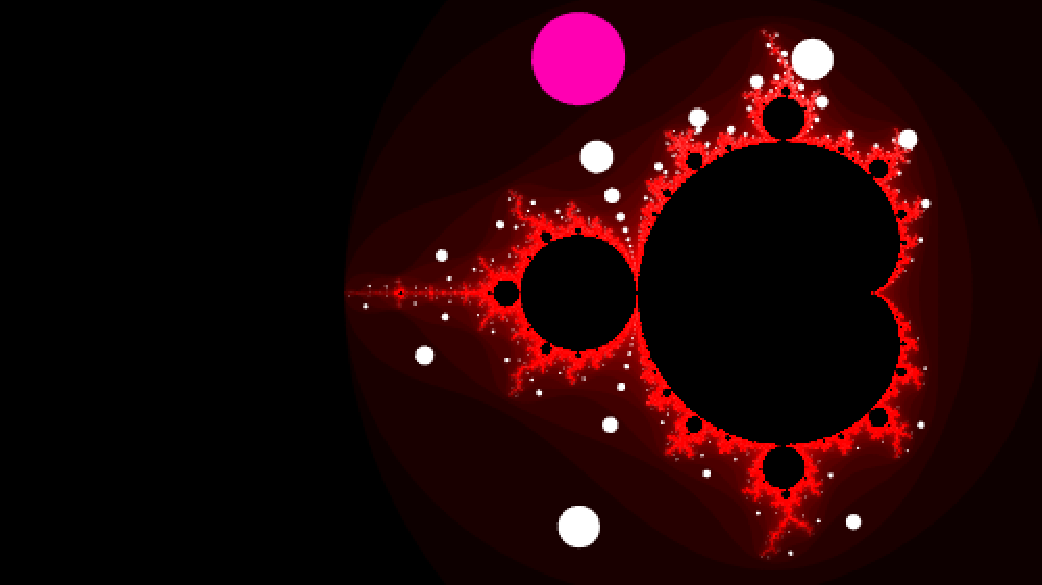
\includegraphics[width=3in, height=3in, keepaspectratio]{../img/fractal/mandelbrot-orbit.pdf}
    \caption{Mandelbrot set}
    \label{fig:mandelbrotOrbit}
  \end{center}
 \end{minipage}
 \begin{minipage}{0.49\hsize}
  \begin{center}
   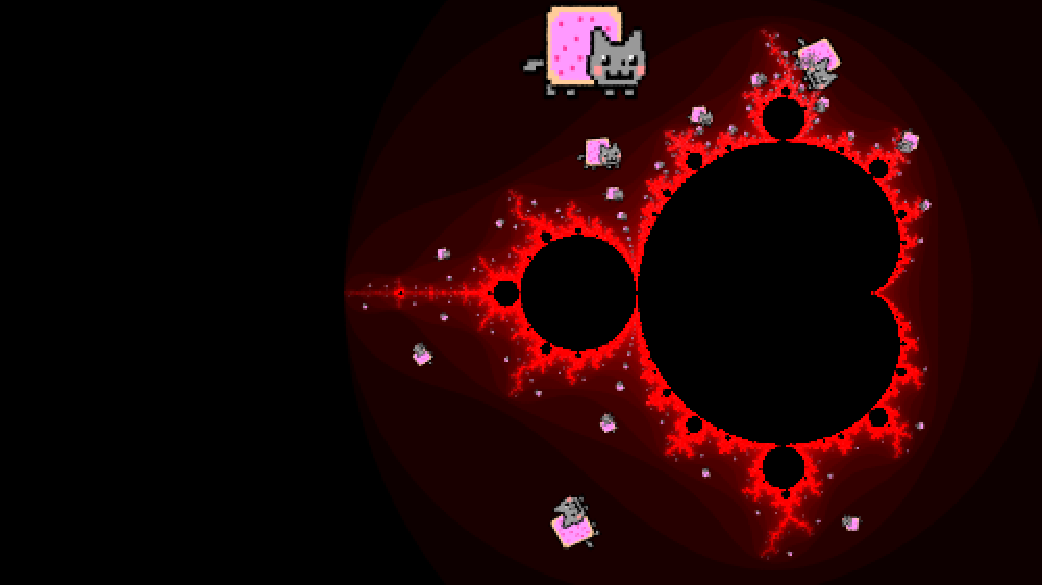
\includegraphics[width=3in, height=3in, keepaspectratio]{../img/fractal/mandelbrot-bitmap.pdf}
   \caption{Mandelbrot set}
   \label{fig:mandelbrotBitmap}
  \end{center}
 \end{minipage}
\end{figure}

\subsection{Iterated Function System}

もう一つ有名なアルゴリズムとして,{\it Iterated Function System (IFS)}が
ある.IFSは点に複数の関数を反復的に作用させることで描画される.

主なアルゴリズムでは,
平面の点をランダムにとり,その点にランダムに選んだ関数を作用させることを
繰り返すことで得られた点を描画する.
シェルピンスキーのギャスケットなどもこの方法でレンダリングすることができる.

IFSに関する書籍としてFractals Everywhere\cite{fractalsEverywhere}がある.
また,並列計算による高速化に関する論文に
\cite{highPerformanceIFS}や,\cite{GPUIFS}がある.

IFSを拡張したフラクタルアートの一種に\emph{フラクタルフレーム}{\it(Fractal
Flame)}\cite{fractalFlame}がある.フラクタルフレームはIFS
に用いる関数にメビウス変換などの非線形変換を用い,美しくレンダリングされ
るようにカラーリングのアルゴリズムにも工夫が加えられている.
図\ref{fig:pseudoKleinian}はフラクタルフレームレンダラのひとつである,
Apophysis 7Xを用いてレンダリングされたフラクタルフレームである.

\begin{figure}[htbp]
  \begin{center}
   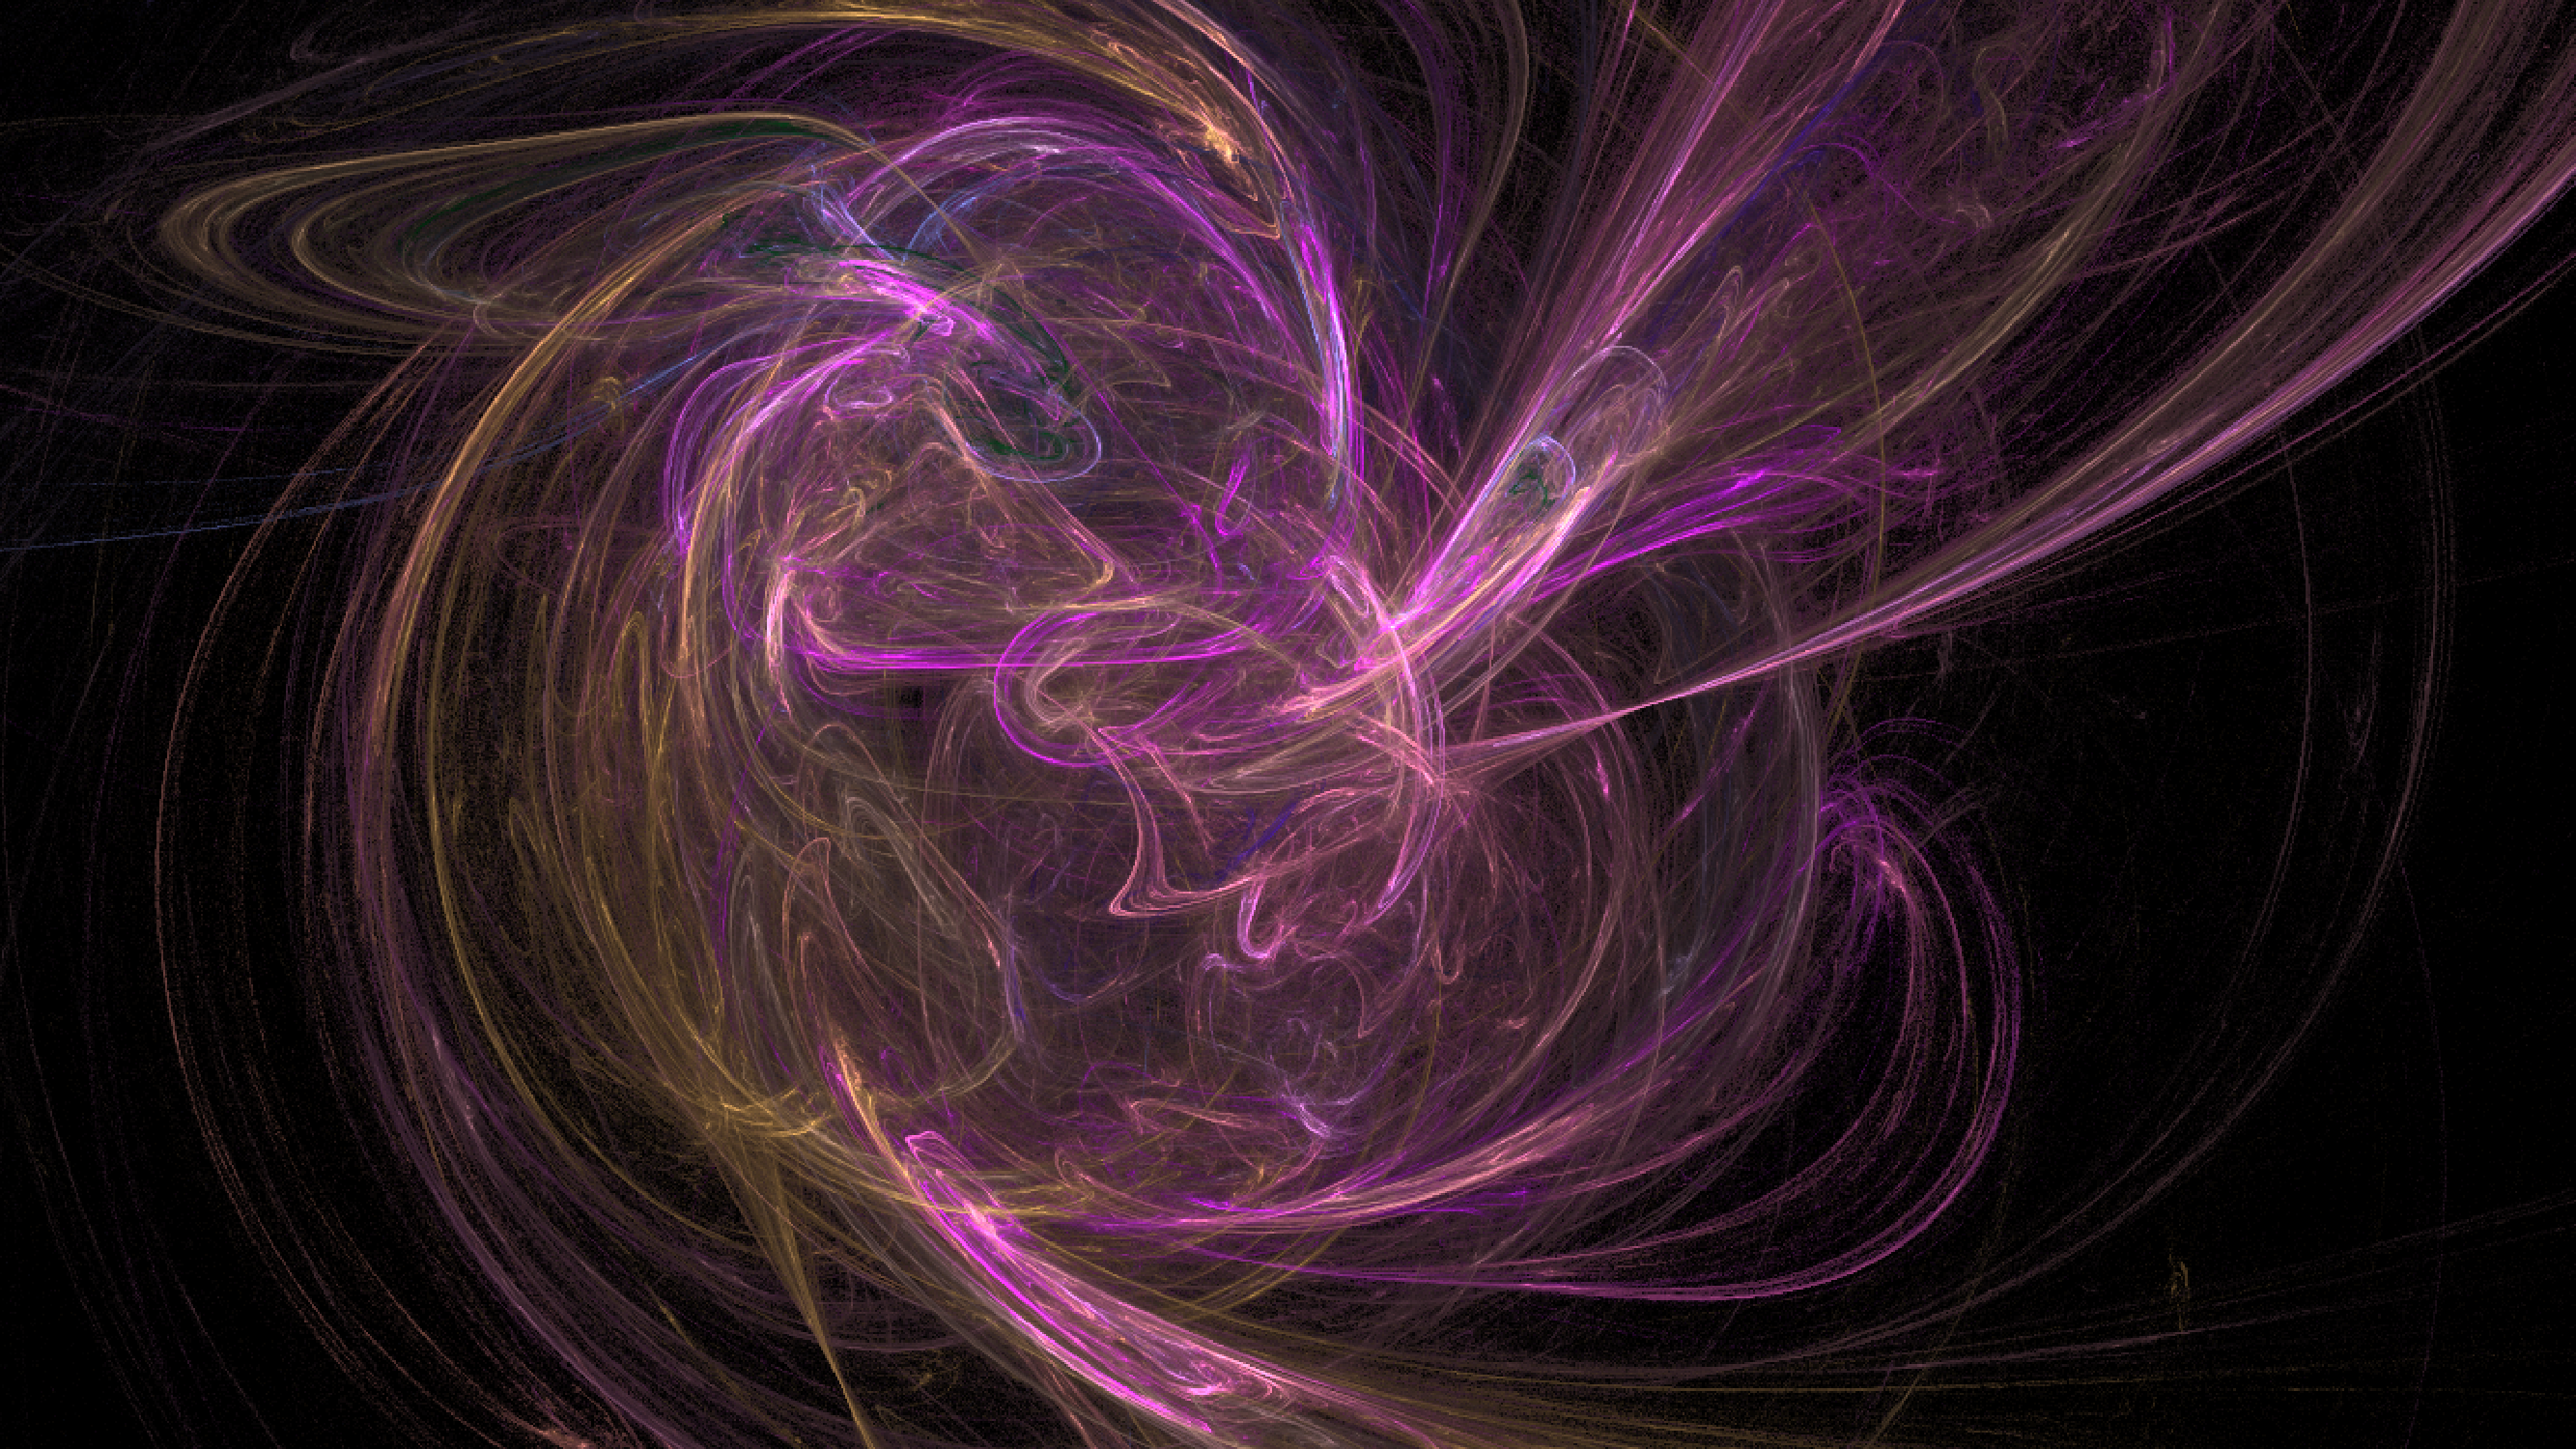
\includegraphics[width=3in, height=3in, keepaspectratio]{../img/fractal/fractalFlame.pdf}
   \caption{Fractal Flame}
   \label{fig:fractalFlame}
  \end{center}
\end{figure}

\clearpage